\documentclass[paper=letter, fontsize=12pt]{article}
\usepackage{geometry}
\geometry{margin=1in}
\usepackage{graphicx}
\graphicspath{{images/}}
\usepackage{amssymb}
\usepackage{enumitem}

%opening
\title{Compsci 571 HW2}
\author{Yilin Gao (yg95)}

\begin{document}

\maketitle
\section{Classifier for Basketball Courts}

\begin{enumerate}[label=(\alph*)]
	\item When running Perceptron algorithm on the dataset, it takes 3 epochs to converge. The decision boundary is $f(x_1, x_2) = -1.05 * x_2 + 1.1 * x_2$. After it converges, the error rate is 0.
	
	The plot of observed data, the decision boundary is:
	
	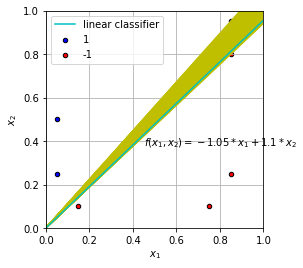
\includegraphics[scale=0.6]{q1a.png}
	
	In the plot there is another linear boundary that goes through the origin to separate the observed data with error = 0.
	
	\item The fully-grown decision tree using Gini index as splitting criterion on the observed data is:
	
	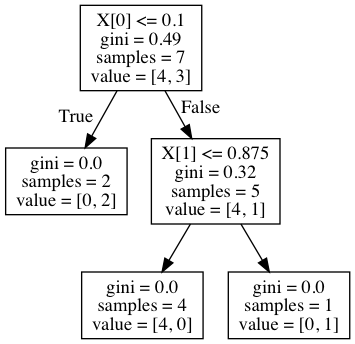
\includegraphics[scale=0.6]{q1b_tree.png}
	
	The error rate is also 0.
	
	The plot of observed data, the decision boundary is:
	
	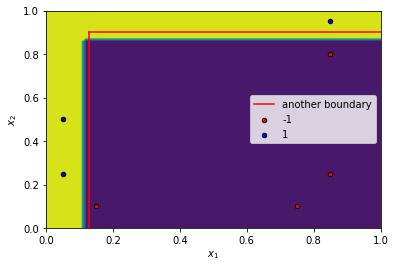
\includegraphics[scale=0.6]{q1b.png}
	
	In the plot there is another decision boundary (in red line) generating the same error rate (0).
	
	\item 
	
	\item 
	
	\item 
	
	\item 
	
	\item 
	
	\item 
	
\end{enumerate}

\section{Variable Importance for Trees and Random Forest}

\begin{enumerate}[label=(\alph*)]
	\item 
	\begin{enumerate}[label=(\roman*)]
		\item 
		The decision stump based on the best split is:
		
		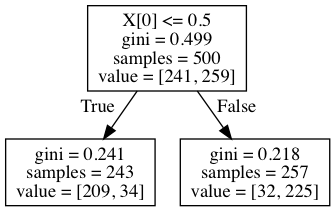
\includegraphics[scale=0.6]{tree_best_split.png}
		
		The decision stump based on the best surrogate split is:
		
		%TODO
		
		\item 
		
		\item 
		The mean least-squares error of predictions on the test data of the decision stump based on the best split is 10.
		
		% TODO
		The mean least-squares error of predictions on the test data of the decision stump based on the best split is 
	\end{enumerate}

	\item 
	\begin{enumerate}[label=(\roman*)]
		\item 
		
		\item 
		
		\item 
	\end{enumerate}

	\item 
	\begin{enumerate}[label=(\roman*)]
		\item 
		
		\item
	\end{enumerate}
\end{enumerate}
\end{document}
